
\section{Description}

The program mainly utilized the concept of arrays to return a working 10-by-10
game board. To improve user experience, visual and audio elements were added to
the program interface. This feature is the significant purpose of using a
resource called \emph{SDL} or https://www.libsdl.org/  Simple DirectMedia Layer,
to render animation, play sound, and showcase creatives.

\begin{table}[H]
    \centering
    \def\arraystretch{2.5}
    \begin{tabular}{ c c c }
        \hline
        Instruction & Definition & Representation \\
        \hline
        O & Pacman & 
\includegraphics[scale=0.1]{assets/pacman_sample.png} \\
        $*$ & Food & 
\includegraphics[scale=0.1]{assets/food_sample.png} \\
        X & Blocks & 
\includegraphics[scale=0.1]{assets/block_sample.png} \\
        \$ & Door & 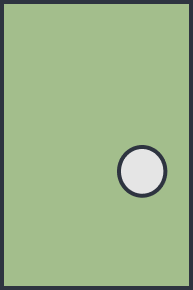
\includegraphics[scale=0.1]{assets/door_sample.png}\\
        \hline
    \end{tabular}
    \caption{The visual representation of symbols in the Ghostless Pacman game}
    \label{tab:1}
\end{table}

Pacman, instead of a a plain 'O' might definitely look more like Pacman. In fact, this Pacman actually munches. Rendering its animation is a feature of the said SDL
library. The same feature allowed the program to display food pieces as
something more delicious than asterisks or any other punctuation, that is,
cherries. The game obstacles that look tougher than 'X', and instead of a dollar
sign for the exit door, an exit door.\\